%% ============================================================
%% Chapter 9 — Linking to Real-world Data Sources and Services
%% Nature Inspired Optimisation for Delivery Problems (2022)
%% Self-contained Beamer lecture notes
%% ============================================================
\documentclass[aspectratio=169,10pt]{beamer}

\usetheme{Madrid}
\usecolortheme{seahorse}
\setbeamertemplate{footline}[frame number]
\setbeamertemplate{navigation symbols}{}

%% --- Packages ---
\usepackage{amsmath,amssymb}
\usepackage{graphicx}
\usepackage{booktabs}
\usepackage{xcolor}
\usepackage{listings}
\usepackage{microtype}
\usepackage{tikz}
\usetikzlibrary{arrows.meta,positioning,shapes.geometric,fit}
\usepackage{hyperref}
\usepackage{array}
\usepackage{colortbl}

\graphicspath{{figures/}}

%% --- Listings style ---
\lstdefinestyle{pycode}{
  language=Python,
  basicstyle=\ttfamily\scriptsize,
  numbers=left,
  numberstyle=\tiny\color{gray},
  frame=single,
  backgroundcolor=\color{gray!7},
  commentstyle=\color{green!50!black}\itshape,
  keywordstyle=\color{blue!70!black}\bfseries,
  stringstyle=\color{orange!80!black},
  showstringspaces=false,
  breaklines=true,
  tabsize=4,
  xleftmargin=1.5em,
  numbersep=6pt,
}

\lstdefinestyle{javacode}{
  language=Java,
  basicstyle=\ttfamily\scriptsize,
  numbers=left,
  numberstyle=\tiny\color{gray},
  frame=single,
  backgroundcolor=\color{blue!4},
  commentstyle=\color{green!45!black}\itshape,
  keywordstyle=\color{violet!80!black}\bfseries,
  stringstyle=\color{orange!70!black},
  showstringspaces=false,
  breaklines=true,
  tabsize=4,
  xleftmargin=1.5em,
  numbersep=6pt,
}

\lstdefinestyle{xmlcode}{
  language=XML,
  basicstyle=\ttfamily\scriptsize,
  numbers=left,
  numberstyle=\tiny\color{gray},
  frame=single,
  backgroundcolor=\color{gray!5},
  commentstyle=\color{green!45!black}\itshape,
  keywordstyle=\color{teal!80!black}\bfseries,
  stringstyle=\color{orange!70!black},
  showstringspaces=false,
  breaklines=true,
  tabsize=2,
  xleftmargin=1.5em,
  numbersep=6pt,
}

%% --- Colours ---
\definecolor{myblue}{RGB}{31,119,180}
\definecolor{myorange}{RGB}{255,127,14}
\definecolor{mygreen}{RGB}{44,160,44}
\definecolor{myred}{RGB}{214,39,40}
\definecolor{mypurple}{RGB}{148,103,189}

%% --- Meta ---
\title[Ch.9 Real-world Data]{Chapter 9: Linking to Real-world Data Sources and Services}
\subtitle{Nature Inspired Optimisation for Delivery Problems (2022)}
\author{Lecture Notes --- Self-contained Edition}
\date{}

%% ============================================================
\begin{document}
%% ============================================================

\begin{frame}
  \titlepage
\end{frame}

%% ────────────────────────────────────────────────────────────
\begin{frame}[allowframebreaks]{Table of Contents}
  \tableofcontents
\end{frame}

%% ============================================================
\section{9.1 Introduction}
%% ============================================================

\begin{frame}[allowframebreaks]{9.1 Introduction --- Why Real-world Data Matters}

  Nature-inspired optimisation algorithms such as Ant Colony Optimisation,
  Genetic Algorithms, and Simulated Annealing are powerful mathematical tools.
  However, their value to practitioners depends critically on two things:
  obtaining \emph{real} input data (actual road distances, not straight-line
  approximations) and presenting \emph{results} in formats that other
  software systems can consume.

  \begin{block}{The Core Challenge}
    Most delivery optimisation algorithms expect, as input, a \emph{distance
    matrix} --- a table of travel distances or journey times between every
    pair of locations.  In the real world, these distances depend on the road
    network, traffic conditions, and vehicle type.  Computing them from
    geographic coordinates requires specialised tools.
  \end{block}

  \medskip
  This chapter introduces three families of tools that close the gap between
  abstract algorithms and real deployments:

  \begin{enumerate}
    \item \textbf{Geocoding} --- converting human-readable addresses into
          latitude/longitude (lat/lon) coordinates.
    \item \textbf{Routing services} --- computing actual road-network distances
          and travel times between pairs of coordinates.
    \item \textbf{Data export} --- writing optimised routes in standard formats
          (KML, GPX, CSV) so they can be displayed in mapping software, loaded
          into GPS devices, or imported into business systems.
  \end{enumerate}

  \begin{alertblock}{Key Insight}
    OpenStreetMap (OSM), launched around 2008, made high-quality geographic
    data freely available to any developer.  Tools such as Nominatim (for
    geocoding) and GraphHopper (for routing) are built on top of OSM data,
    enabling sophisticated real-world solvers without commercial licensing costs.
  \end{alertblock}

  \framebreak

  \textbf{The Overall Integration Pipeline}

  \medskip
  The diagram below shows how the components in this chapter fit together.
  A sequence of address strings is converted to coordinates by the geocoder,
  then a routing service computes the pairwise distance/duration matrix, the
  optimiser finds a good route, and finally an export service writes the result
  to a file format suitable for visualisation or navigation.

  \begin{center}
    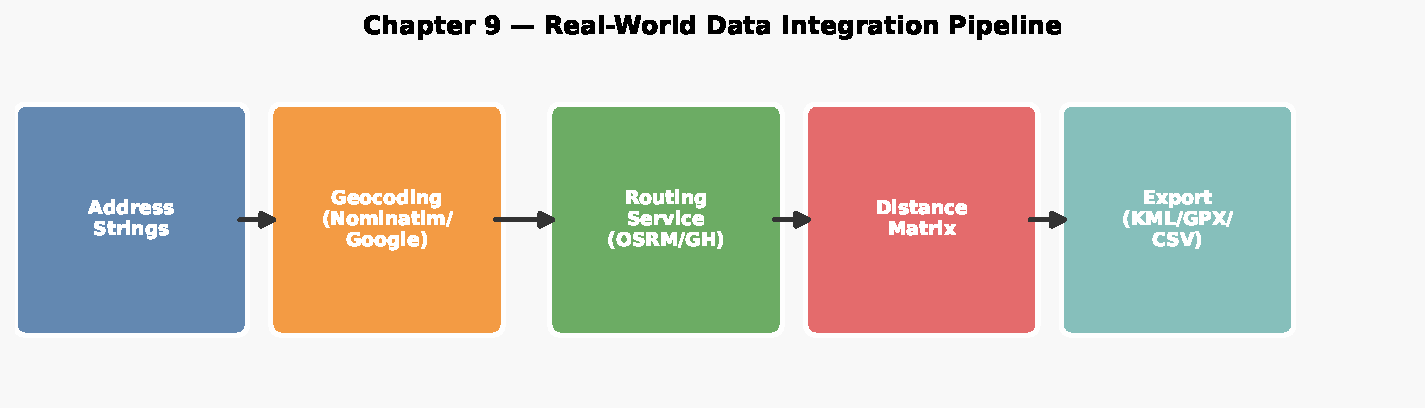
\includegraphics[width=0.95\textwidth]{fig_pipeline}
  \end{center}

  Each component is designed as a \emph{swappable module}: the book's Java
  code uses interfaces and abstract classes so that, for example, the Nominatim
  geocoder can be replaced by a Google Maps geocoder without touching the rest
  of the system.  This design principle is equally applicable in Python.

\end{frame}

%% ============================================================
\section{9.2 Geocoding}
%% ============================================================

\begin{frame}[allowframebreaks]{9.2 Geocoding --- Addresses to Coordinates}

  \textbf{What is geocoding?}

  Geocoding is the process of converting a human-readable location description
  --- such as a postal address, a place name, or a postcode --- into a pair of
  geographic coordinates: \emph{latitude} (lat) and \emph{longitude} (lon).
  These coordinates are numbers that pin a location precisely on the surface
  of the Earth.

  \begin{block}{Notation: Latitude and Longitude}
    \textbf{Latitude} is measured in degrees from $-90°$ (South Pole) to
    $+90°$ (North Pole), where $0°$ is the Equator.  A positive value means
    north of the Equator.

    \textbf{Longitude} is measured in degrees from $-180°$ to $+180°$, where
    $0°$ is the Prime Meridian (Greenwich, UK).  A negative value means west.

    Example: Edinburgh Napier University, Merchiston Campus is at approximately
    $\text{lat} = 55.93°$N, $\text{lon} = -3.21°$W.
  \end{block}

  \medskip
  There are two directions of geocoding:

  \begin{itemize}
    \item \textbf{Forward geocoding}: given an address string, return
          coordinates.  This is the most common need --- a spreadsheet of
          delivery addresses must be converted to lat/lon before distances
          can be computed.
    \item \textbf{Reverse geocoding}: given coordinates, return the nearest
          address label.  This is used when an optimiser returns a solution
          expressed in coordinates and a human-readable label is needed for
          the output.
  \end{itemize}

  \begin{center}
    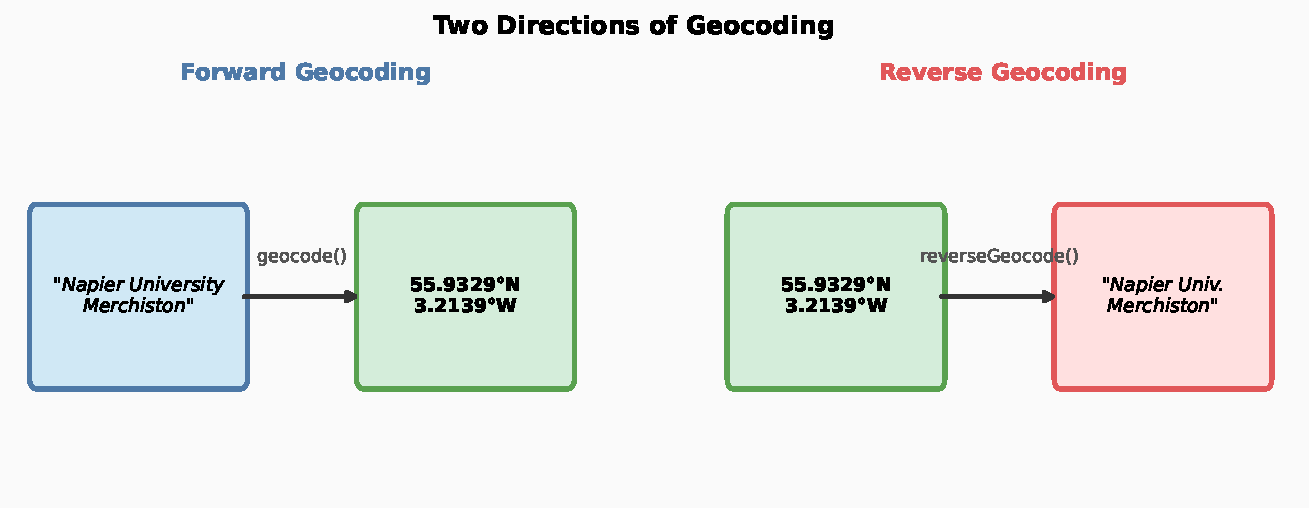
\includegraphics[width=0.82\textwidth]{fig_forward_reverse}
  \end{center}

  \framebreak

  \textbf{Practical Considerations}

  \medskip
  A single address string can be ambiguous.  For example, the string
  \texttt{"High Street, Edinburgh"} could match dozens of streets.  A robust
  geocoder handles this by:
  \begin{itemize}
    \item Returning the most \emph{important} match (e.g., the one with the
          highest population or the most prominent place type).
    \item Accepting structured input (street, city, postcode) to reduce
          ambiguity.
    \item Returning a \emph{confidence score} so the application can flag
          uncertain results for human review.
  \end{itemize}

  \medskip
  For \emph{reverse geocoding}, a coordinate may lie in the middle of a field
  far from any address.  Two strategies exist:
  \begin{enumerate}
    \item Return the \emph{nearest label}, regardless of distance.  This
          always gives an answer but may be geographically misleading.
    \item Return the nearest label only if it is \emph{within a threshold
          distance} (e.g., 10 metres).  If no label is close enough, report
          ``not found''.
  \end{enumerate}
  The book implements both strategies; the second (threshold-based) approach
  is generally safer in production.

\end{frame}

%% ────────────────────────────────────────────────────────────
\begin{frame}[allowframebreaks]{9.2 A Simple Geocoder --- NapierLoc}

  Before connecting to web services, the book introduces a \emph{simple
  hand-crafted geocoder} called \texttt{NapierLoc}, which stores a hard-coded
  list of a few Edinburgh university campuses.  While trivially small, it
  illustrates the key design patterns used throughout this chapter.

  \begin{block}{The Geocoder Interface (Java)}
    The book defines a Java \texttt{Geocoder} interface with exactly two
    methods:
    \begin{itemize}
      \item \texttt{geocode(String label)} --- takes an address string,
            returns a \texttt{LatLon} object (latitude, longitude).
      \item \texttt{reverseGeocode(LatLon p)} --- takes a \texttt{LatLon}
            point, returns the nearest label string.
    \end{itemize}
    All geocoders in the system implement this same interface.  This means
    the optimisation algorithm never needs to know \emph{which} geocoder it
    is using --- it simply calls \texttt{geocode()} and gets a result.
  \end{block}

  \begin{center}
    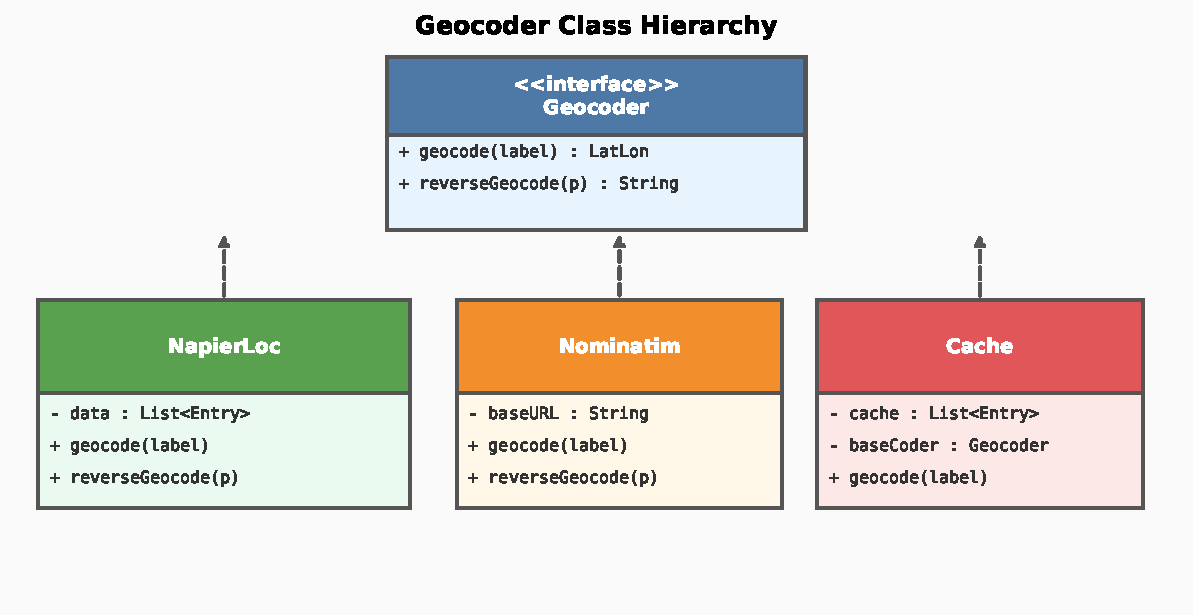
\includegraphics[width=0.75\textwidth]{fig_geocoder_hierarchy}
  \end{center}

  \framebreak

  \textbf{How NapierLoc Works}

  \medskip
  The \texttt{NapierLoc} class stores a list of \texttt{Entry} objects.
  Each \texttt{Entry} holds one label--coordinate mapping, for example:

  \begin{itemize}
    \item \texttt{"Napier University, Merchiston"} $\rightarrow$
          $(55.9329,\; -3.2139)$
    \item \texttt{"Napier University, Craiglockhart"} $\rightarrow$
          $(55.9180,\; -3.2397)$
    \item \texttt{"Napier University, Sighthill"} $\rightarrow$
          $(55.9242,\; -3.2885)$
  \end{itemize}

  \medskip
  The \texttt{geocode()} method performs a \emph{linear search} through
  the list looking for an exact label match.  If found, it returns the
  associated coordinates; otherwise it returns \texttt{null}.

  The \texttt{reverseGeocode()} method computes the \emph{Euclidean distance}
  (in coordinate space) from the query point to every stored location, and
  returns the label of the closest one.

  \begin{alertblock}{Scalability Warning}
    Both methods have time complexity $\Theta(n)$ --- that is, proportional
    to $n$ (nu), the number of entries.  Here $n$ is small (three campuses),
    so this is fine.  For large datasets, such as the entire UK postcode
    database (around 1.7~million entries), a hierarchical spatial data
    structure (e.g., a k-d tree) would be needed to keep searches fast.
    $\Theta$ (Theta, meaning ``exact order of growth'') is used to say the
    running time grows at exactly this rate --- not faster, not slower.
  \end{alertblock}

\end{frame}

%% ────────────────────────────────────────────────────────────
\begin{frame}[allowframebreaks]{9.2 Web-based Geocoding --- Nominatim}

  The simple \texttt{NapierLoc} geocoder only knows three locations.  For
  real delivery problems we need a geocoder that can handle \emph{any} valid
  UK address.  The solution is to connect to a \emph{web-based geocoding
  service}.

  \begin{block}{What a Web Geocoding Service Provides}
    \begin{itemize}
      \item \textbf{Coverage}: handles millions of addresses across entire
            countries or the world.
      \item \textbf{Parsing}: interprets free-form address strings entered
            by end users, even with typos or abbreviated forms.
      \item \textbf{Updating}: the service provider keeps the data current;
            the application developer does not need to maintain any geographic
            database.
    \end{itemize}
  \end{block}

  \medskip
  \textbf{Nominatim} is the official geocoding service for
  OpenStreetMap (OSM).  It is free to use and is accessed via a simple
  HTTP request.  The URL format for a forward geocoding query is:

  \begin{center}
    \texttt{https://nominatim.openstreetmap.org/search?q=\{address\}\&format=xml}
  \end{center}

  \noindent
  where \texttt{\{address\}} is a URL-encoded address string.
  Nominatim returns an XML document containing one or more matching places.

  \framebreak

  \textbf{Reading the Nominatim XML Response}

  \medskip
  The XML response looks like this (simplified):

  \begin{center}
    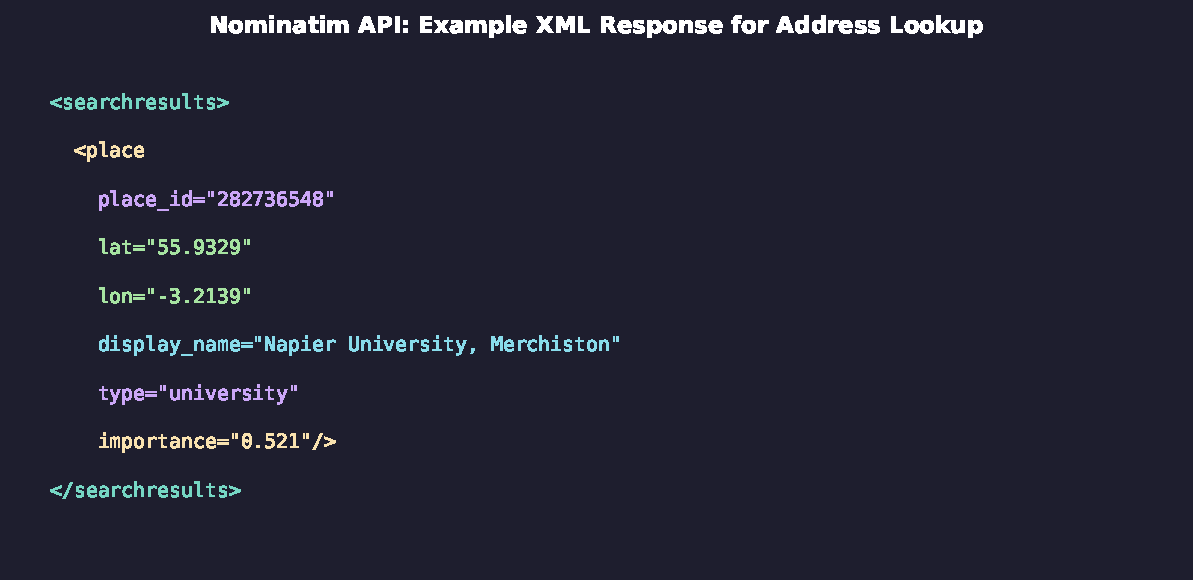
\includegraphics[width=0.72\textwidth]{fig_nominatim_xml}
  \end{center}

  \medskip
  The key fields are:
  \begin{itemize}
    \item \texttt{lat} and \texttt{lon}: the decimal-degree coordinates of
          the matched location.
    \item \texttt{display\_name}: a human-readable description of the match.
    \item \texttt{importance}: a score (0 to 1) reflecting how prominent this
          place is; higher-importance matches should be preferred when multiple
          results are returned.
    \item \texttt{type}: the category of place (e.g., ``university'',
          ``road'', ``city'').
  \end{itemize}

  The application code must parse this XML (using a suitable library),
  extract the first result's \texttt{lat} and \texttt{lon} values, and
  return them as a \texttt{LatLon} object.

  \framebreak

  \textbf{Caching Geocoding Requests --- The Cache Class}

  \medskip
  A freely provided web service such as Nominatim imposes
  \emph{usage limits}.  Nominatim's policy (as of 2022) allows at most
  one request per second from any single client.  In an optimisation
  experiment that calls the geocoder hundreds or thousands of times,
  this could be a bottleneck.  More importantly, repeatedly geocoding
  the same address wastes network bandwidth and may violate the service's
  fair-use policy.

  The \emph{Cache} design pattern solves this problem.  The \texttt{Cache}
  class wraps any \texttt{Geocoder} and stores results in memory.
  When a request arrives, the cache first checks its stored results:

  \begin{center}
    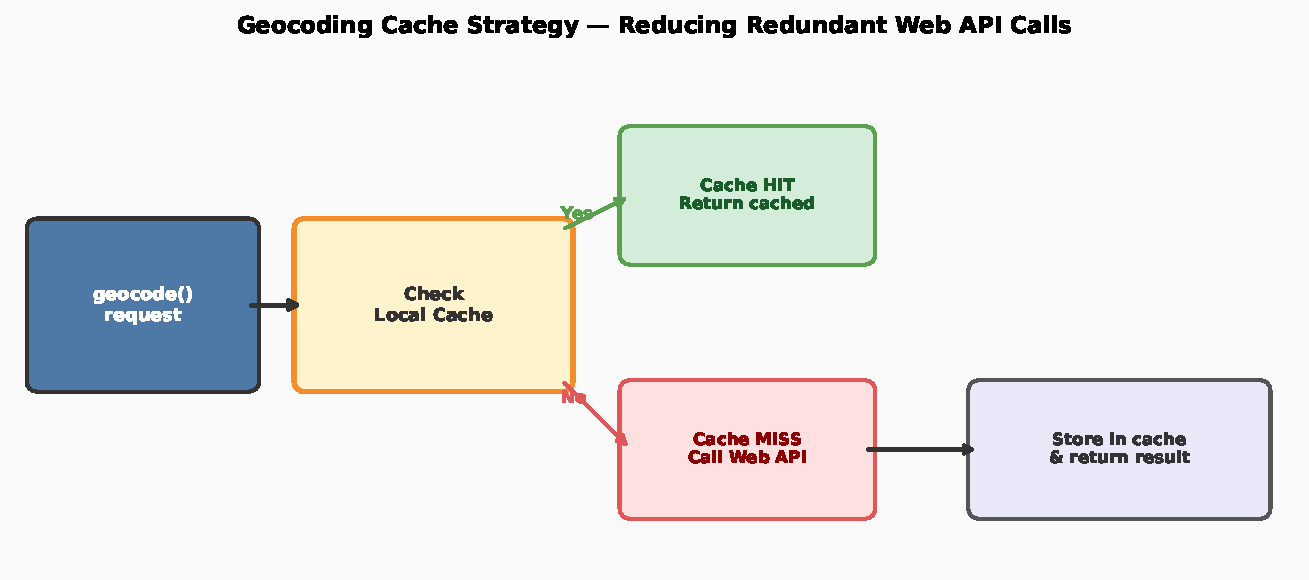
\includegraphics[width=0.90\textwidth]{fig_cache_strategy}
  \end{center}

  \framebreak

  \textbf{How the Cache Works (Detail)}

  \begin{itemize}
    \item \textbf{Cache hit}: if the requested label is already in the
          internal list, return the stored coordinates immediately.  No
          web request is made.
    \item \textbf{Cache miss}: if the label is not in the cache, delegate
          to the wrapped \texttt{Geocoder} (e.g., Nominatim), get the result,
          store it in the cache, and return it.
  \end{itemize}

  \medskip
  For reverse geocoding, the cache uses a \emph{distance threshold}:
  if a stored point is within \texttt{REVERSE\_THRESHOLD} degrees of
  the query point (set to \texttt{0.01} in the book's code), the cached
  label is returned.  Otherwise, the web service is consulted.

  \begin{block}{The Cache as a Geocoder Decorator}
    The \texttt{Cache} class itself implements the \texttt{Geocoder}
    interface.  The rest of the application sees it as just another
    geocoder.  This is the \emph{Decorator} design pattern: behaviour is
    added (caching) without modifying the original class.  To use the cache:
    \texttt{Geocoder gc = new Cache(new Nominatim());}
  \end{block}

  \begin{alertblock}{Key Insight}
    Caching is especially important during development and testing.  When
    experimenting with an optimisation algorithm, the same set of addresses
    is geocoded repeatedly across many runs.  A cache means the web service
    is contacted only once per unique address for the entire session.
  \end{alertblock}

  \framebreak

  \textbf{Hosting Your Own Nominatim Instance}

  \medskip
  For large-scale projects --- such as a logistics company running
  thousands of experiments per day --- connecting to the public Nominatim
  service is impractical due to rate limits.  An alternative is to
  \emph{download and host Nominatim locally} on the developer's own hardware.

  \begin{itemize}
    \item Nominatim is open-source software that can be installed on any
          Linux server.
    \item OSM data for a country or region can be downloaded as a
          \texttt{.osm.pbf} file (typically a few gigabytes for the UK).
    \item Once installed, a local Nominatim instance has no rate limits
          and does not require an internet connection at query time.
  \end{itemize}

  This approach provides:
  \begin{enumerate}
    \item \textbf{Speed}: local queries take milliseconds rather than the
          100--500~ms typical of a public API.
    \item \textbf{Reliability}: no dependency on third-party uptime.
    \item \textbf{Privacy}: address data never leaves the organisation's
          network.
  \end{enumerate}

\end{frame}

%% ────────────────────────────────────────────────────────────
\begin{frame}[fragile]{Python: Geocoding with geopy + Nominatim}

  The Python \texttt{geopy} library provides a clean interface to Nominatim
  (and many other geocoding services) without writing raw HTTP requests.
  The example below geocodes two Edinburgh addresses, prints their coordinates,
  and then reverse-geocodes the first result to verify.

\begin{lstlisting}[style=pycode, caption={Forward and reverse geocoding using geopy}]
from geopy.geocoders import Nominatim
from geopy.extra.rate_limiter import RateLimiter
import time

# Create a geolocator.  The user_agent string identifies your application
# to Nominatim -- it must be unique and not "test" or "myapp".
geolocator = Nominatim(user_agent="delivery_optimiser_v1")

# RateLimiter wraps the geocode function to enforce a 1-second pause
# between requests, respecting Nominatim's usage policy.
geocode = RateLimiter(geolocator.geocode, min_delay_seconds=1)

# --- Forward geocoding: address string -> (latitude, longitude) ---
addresses = [
    "10 Colinton Road, Edinburgh",
    "Scottish Vintage Bus Museum, Fife",
]

locations = {}
for addr in addresses:
    loc = geocode(addr)
    if loc is not None:
        locations[addr] = (loc.latitude, loc.longitude)
        print(f"  {addr}")
        print(f"    -> lat={loc.latitude:.5f}, lon={loc.longitude:.5f}")
    else:
        print(f"  NOT FOUND: {addr}")

# --- Reverse geocoding: (latitude, longitude) -> address label ---
lat, lon = list(locations.values())[0]
result = geolocator.reverse(f"{lat}, {lon}", language="en")
print(f"\nReverse geocode ({lat:.4f}, {lon:.4f}):")
print(f"  -> {result.address}")
\end{lstlisting}

  \begin{alertblock}{Usage Policy Reminder}
    Nominatim is a free community service.  Always use \texttt{RateLimiter}
    (or an equivalent pause), set a descriptive \texttt{user\_agent}, and
    cache results to avoid repeated queries.  Commercial use at scale requires
    a commercial geocoding provider (e.g., Google Maps Platform, Here Maps).
  \end{alertblock}

\end{frame}

%% ────────────────────────────────────────────────────────────
\begin{frame}[fragile]{Python: Building a Simple In-memory Geocoder Cache}

  The following Python class mirrors the book's Java \texttt{Cache} design.
  It wraps any \texttt{geopy} geolocator and stores results in a dictionary,
  so each unique address is only sent to the web service once.

\begin{lstlisting}[style=pycode, caption={A simple geocoding cache in Python}]
from geopy.geocoders import Nominatim
from geopy.extra.rate_limiter import RateLimiter
import math

class GeocoderCache:
    """
    Wraps a geopy geolocator with an in-memory cache.
    Forward cache: { address_string -> (lat, lon) }
    Reverse cache: list of ( (lat, lon), label ) pairs
    """
    REVERSE_THRESHOLD = 0.01  # degrees; ~1 km at UK latitudes

    def __init__(self, geolocator, min_delay=1.0):
        self._geocode = RateLimiter(
            geolocator.geocode, min_delay_seconds=min_delay
        )
        self._reverse = RateLimiter(
            geolocator.reverse, min_delay_seconds=min_delay
        )
        self._fwd_cache = {}       # address -> (lat, lon)
        self._rev_cache = []       # list of ((lat,lon), label)

    def geocode(self, address: str):
        """Forward geocode: return (lat, lon) or None."""
        if address in self._fwd_cache:
            return self._fwd_cache[address]          # cache hit
        loc = self._geocode(address)                 # web call
        if loc is None:
            return None
        result = (loc.latitude, loc.longitude)
        self._fwd_cache[address] = result
        self._rev_cache.append((result, address))    # also cache reverse
        return result

    def reverse_geocode(self, lat: float, lon: float) -> str:
        """Reverse geocode: return nearest label or 'Not found'."""
        # Search the local cache first
        best_dist, best_label = float('inf'), None
        for (clat, clon), label in self._rev_cache:
            d = math.sqrt((lat - clat)**2 + (lon - clon)**2)
            if d < best_dist:
                best_dist, best_label = d, label
        if best_dist <= self.REVERSE_THRESHOLD:
            return best_label                        # cache hit
        # Cache miss: call the web service
        loc = self._reverse(f"{lat}, {lon}", language="en")
        label = loc.address if loc else "Not found"
        self._rev_cache.append(((lat, lon), label))
        return label
\end{lstlisting}

\end{frame}

%% ============================================================
\section{9.3 Using Routing Services}
%% ============================================================

\begin{frame}[allowframebreaks]{9.3 Routing Services --- Road-network Distances}

  \textbf{Why straight-line distances are not enough}

  \medskip
  A common shortcut in early implementations of routing algorithms is to
  use the \emph{Haversine formula} to compute straight-line (``as the crow
  flies'') distances between coordinates.  While simple, this leads to
  inaccurate results in practice:

  \begin{itemize}
    \item Roads follow bends, hills, and rivers --- they are never perfectly
          straight.
    \item A short straight-line distance may correspond to a very long drive
          if a river or motorway junction separates the two points.
    \item Journey \emph{time} depends on speed limits, traffic signals, and
          traffic conditions, not just distance.
  \end{itemize}

  A \emph{routing service} computes distances and travel times along the
  actual road network, using graph search algorithms (typically variants of
  Dijkstra's algorithm or A*) applied to a road-network graph derived from
  OSM data.

  \begin{block}{What a Routing Service Returns (a Journey object)}
    For a given pair of start and end coordinates, a routing service returns:
    \begin{itemize}
      \item \textbf{Distance} (km): the road-network distance.
      \item \textbf{Travel time} (ms or minutes): the estimated journey duration.
      \item \textbf{Path}: a sequence of lat/lon waypoints defining the exact
            route to follow on the road network.
    \end{itemize}
  \end{block}

  \framebreak

  \textbf{The RoutingEngine Abstract Class}

  \medskip
  Just as the \texttt{Geocoder} interface made geocoders swappable,
  the book defines a \texttt{RoutingEngine} abstract class so that
  the choice of routing back-end (local library vs.\ web API) does not
  affect the rest of the application.

  The single abstract method is:
  \begin{center}
    \texttt{Journey findRoute(LatLon start, LatLon end, HashMap<String,String> options)}
  \end{center}

  The \texttt{options} map allows passing engine-specific parameters
  (such as vehicle type or data file location) without changing the
  method signature.  Three concrete options keys are defined:
  \begin{itemize}
    \item \texttt{OPTION\_DATA\_DIR}: directory containing the OSM road
          data file.
    \item \texttt{OPTION\_OSM\_FILE}: the filename of the \texttt{.osm}
          data file.
    \item \texttt{OPTION\_MODE}: travel mode, e.g., \texttt{"car"},
          \texttt{"bike"}, \texttt{"foot"}.
  \end{itemize}

  \begin{center}
    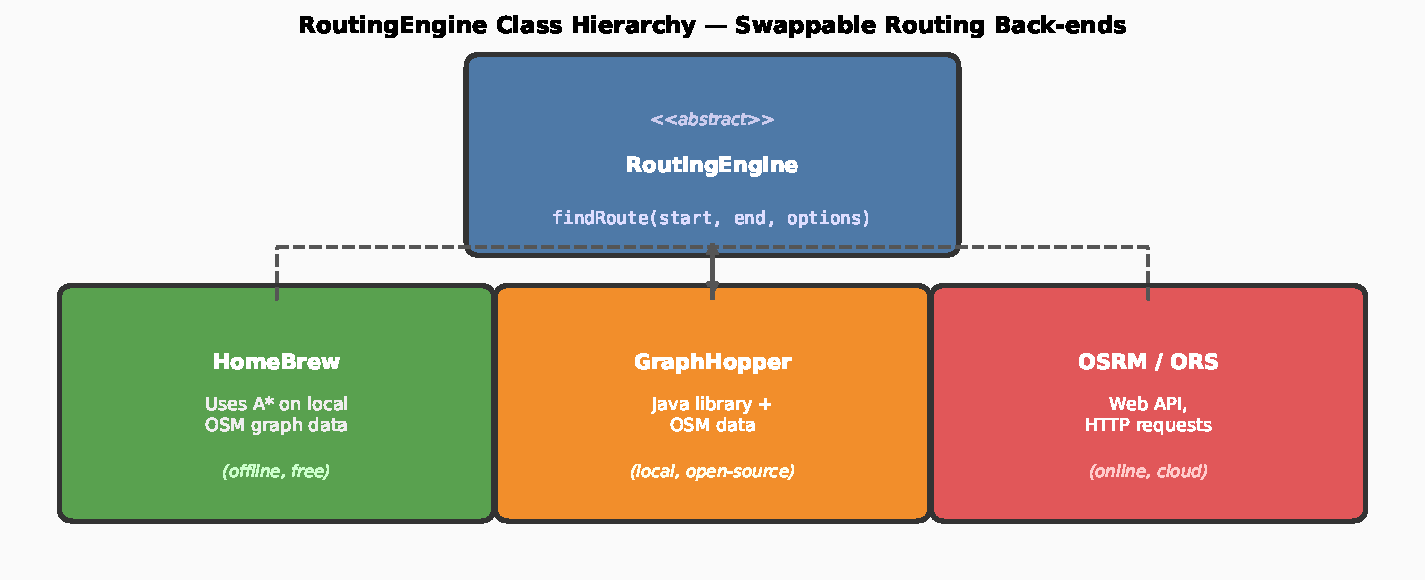
\includegraphics[width=0.88\textwidth]{fig_routing_architecture}
  \end{center}

  \framebreak

  \textbf{Three Routing Back-ends}

  \medskip
  The book implements and compares three concrete routing engines:

  \begin{enumerate}
    \item \textbf{HomeBrew}: a custom Java implementation that reads an OSM
          XML file, builds an in-memory road graph, and applies the A*
          algorithm to find the shortest path.  It is the most instructive
          to study (the book's Chapter~8 builds it from scratch) but the
          slowest in practice.

    \item \textbf{GraphHopper}: an open-source Java routing library built
          on top of OSM data.  It is much faster than HomeBrew because it
          pre-processes the road graph for speed.  GraphHopper supports
          multiple travel modes (car, bike, foot) and can run entirely
          offline.

    \item \textbf{OSRM} (Open Source Routing Machine) or
          \textbf{OpenRouteService (ORS)}: web APIs that accept HTTP requests
          and return JSON responses.  These are suitable when the client
          machine does not have enough RAM to load a full country-level road
          graph, or when a reliable internet connection is available.
  \end{enumerate}

  The key advantage of the abstract class design is that all three engines
  produce the same \texttt{Journey} object.  The optimisation algorithm
  is completely unaware of which engine is in use.

  \framebreak

  \textbf{GraphHopper in Practice}

  \medskip
  GraphHopper (GH) is recommended for most research use-cases because it:
  \begin{itemize}
    \item Works offline using a downloaded OSM file (no API keys required).
    \item Handles a full country-level road graph in a few hundred MB of RAM.
    \item Returns results in milliseconds, fast enough for optimisation
          experiments that call \texttt{findRoute()} millions of times.
  \end{itemize}

  When first called, the GH implementation checks whether the road graph
  has already been initialised.  If not, it loads the OSM file and builds
  the routing graph (a one-time cost taking a few seconds).  Subsequent
  calls reuse the loaded graph.

  \begin{exampleblock}{Worked Example: Edinburgh to Glasgow by Car}
    Using a Scotland OSM file and GraphHopper in car mode:
    \begin{itemize}
      \item Start: $55.9329°$N, $3.2139°$W (Napier University, Edinburgh)
      \item End: $55.8617°$N, $4.2583°$W (University of Glasgow)
      \item Road distance: $\approx 74$~km
      \item Estimated travel time: $\approx 65$~minutes (by car, no traffic)
      \item Path: a sequence of $\sim$250 waypoints tracing the M8 motorway
    \end{itemize}
    A straight-line calculation gives only $\approx 65$~km, underestimating
    the road distance by about 12\%.
  \end{exampleblock}

\end{frame}

%% ────────────────────────────────────────────────────────────
\begin{frame}[allowframebreaks]{9.3 Building the Distance Matrix}

  For delivery optimisation, we need pairwise distances between all
  locations --- not just one pair.  If there are $n$ (the number of
  locations) delivery stops plus one depot, there are
  $n(n+1)$ ordered pairs (since distance from A to B may differ from
  B to A if one-way streets exist).

  \begin{block}{Distance Matrix Definition}
    Let $D$ be an $n \times n$ matrix where $D_{ij}$ (read: ``D sub i j'')
    is the road-network travel distance (or time) from location $i$ to
    location $j$.  In most road networks:
    \[
      D_{ij} \approx D_{ji}
    \]
    but strict equality does not hold in general (one-way streets,
    turn penalties).  The diagonal entries $D_{ii} = 0$ (distance from a
    location to itself is zero).
  \end{block}

  \medskip
  \textbf{How to read this formula:}  $D_{ij}$ means ``the element in row $i$,
  column $j$ of matrix $D$''.  The subscripts $i$ and $j$ are indices:
  $i$ identifies the \emph{origin} location and $j$ the
  \emph{destination} location.  For a problem with $n=5$ stops, $D$ is a
  $5 \times 5$ table containing 25 entries.

  \begin{center}
    
\includegraphics[width=0.82\textwidth]{fig_distance_matrix}
  \end{center}

  \framebreak

  \textbf{Computing the Distance Matrix Efficiently}

  \medskip
  A naive approach calls \texttt{findRoute()} once for every ordered pair,
  which means $n^2$ routing queries.  For $n = 100$ stops this is
  10,000 queries --- fine for an offline library, but potentially slow for
  a web API.

  Several web APIs (OSRM, OpenRouteService) accept a \emph{matrix endpoint}
  that computes all $n^2$ pairs in a single HTTP request, much more
  efficiently than $n^2$ separate requests.

  \begin{exampleblock}{Matrix Computation: 5 Scottish Cities}
    \centering
    \begin{tabular}{l|rrrrr}
      \toprule
      (km) & Edin. & Glasg. & Stirl. & Perth & Dundee \\
      \midrule
      Edinburgh & 0  & 74 & 56 & 60 &  93 \\
      Glasgow   & 74 &  0 & 36 & 88 & 121 \\
      Stirling  & 56 & 36 &  0 & 52 &  85 \\
      Perth     & 60 & 88 & 52 &  0 &  34 \\
      Dundee    & 93 &121 & 85 & 34 &   0 \\
      \bottomrule
    \end{tabular}

    \medskip
    \small Road distances (approximate) from OSRM.
    Note: the matrix is approximately symmetric but not exactly
    (e.g., motorway routing may differ in each direction).
  \end{exampleblock}

  \medskip
  Once the distance matrix is computed, it is stored in memory.  The
  optimisation algorithm then looks up $D_{ij}$ in O(1) time (constant
  time, meaning one memory access) rather than making a fresh routing
  request every time it evaluates a route.

  \begin{alertblock}{Key Insight}
    Pre-computing and caching the full distance matrix is the single most
    important performance optimisation when using routing services.  The
    matrix computation is a one-time cost; all subsequent evaluations by
    the optimisation algorithm are table lookups.
  \end{alertblock}

\end{frame}

%% ────────────────────────────────────────────────────────────
\begin{frame}[fragile]{Python: Routing with OSRM Table API}

  The OSRM \emph{table} endpoint computes a complete distance or duration
  matrix in one HTTP request.  The example below builds a duration matrix
  (in seconds) for five Scottish cities using the public OSRM demo server.

\begin{lstlisting}[style=pycode, caption={Distance/duration matrix via OSRM Table API}]
import requests
import numpy as np

# Coordinates: [longitude, latitude] format for OSRM
cities = {
    "Edinburgh": (55.9329, -3.2139),
    "Glasgow":   (55.8617, -4.2583),
    "Stirling":  (56.1165, -3.9369),
    "Perth":     (56.3964, -3.4370),
    "Dundee":    (56.4621, -2.9707),
}

names = list(cities.keys())
coords = list(cities.values())

# Build the OSRM coordinate string: lon,lat;lon,lat;...
coord_str = ";".join(f"{lon},{lat}" for lat, lon in coords)

# OSRM table API endpoint (public demo server -- replace with own instance
# for production; demo server has rate limits)
url = (f"http://router.project-osrm.org/table/v1/driving/{coord_str}"
       f"?annotations=duration,distance")

resp = requests.get(url, timeout=15)
data = resp.json()

# Extract duration matrix (seconds) and distance matrix (metres)
dur_matrix  = np.array(data["durations"])   # n x n, seconds
dist_matrix = np.array(data["distances"])   # n x n, metres

print("Duration matrix (minutes):")
print(f"{'':12}", end="")
for n in names:
    print(f"{n[:6]:>8}", end="")
print()
for i, row_name in enumerate(names):
    print(f"{row_name:12}", end="")
    for j in range(len(names)):
        val = dur_matrix[i, j] / 60.0      # convert seconds -> minutes
        print(f"{val:8.1f}", end="")
    print()
\end{lstlisting}

\end{frame}

%% ────────────────────────────────────────────────────────────
\begin{frame}[fragile]{Python: Routing with GraphHopper (Python Client)}

  If an internet connection is unavailable, GraphHopper can be run as a
  local server with a downloaded OSM file.  The Python \texttt{graphh}
  package provides a convenient client.

\begin{lstlisting}[style=pycode, caption={Single route query with GraphHopper local server}]
# pip install graphh
# Assumes GraphHopper is running locally: java -jar graphhopper.jar ...
import requests, json

GH_URL = "http://localhost:8989/route"   # local GraphHopper server

def get_route(lat1, lon1, lat2, lon2, vehicle="car"):
    """
    Query a locally running GraphHopper server for the route
    from (lat1, lon1) to (lat2, lon2).
    Returns: dict with 'distance_km' and 'time_min'.
    """
    params = {
        "point": [f"{lat1},{lon1}", f"{lat2},{lon2}"],
        "vehicle": vehicle,
        "locale": "en",
        "calc_points": "false",   # omit waypoints for speed
        "type": "json",
    }
    resp = requests.get(GH_URL, params=params, timeout=10)
    resp.raise_for_status()
    data = resp.json()

    path = data["paths"][0]
    return {
        "distance_km": path["distance"] / 1000.0,
        "time_min":    path["time"] / 60000.0,   # ms -> minutes
    }

# Example: Edinburgh Napier -> Scottish Vintage Bus Museum, Fife
r = get_route(55.9329, -3.2139, 56.1503, -3.3521)
print(f"Distance: {r['distance_km']:.1f} km")
print(f"Time:     {r['time_min']:.1f} min")
\end{lstlisting}

\end{frame}

%% ============================================================
\section{9.4 Exporting Data}
%% ============================================================

\begin{frame}[allowframebreaks]{9.4 Exporting Data --- Standard GIS Formats}

  After the optimisation algorithm finds a good delivery route, the result
  must be communicated to humans and to other software systems.
  Three widely-used geospatial data formats make routes readable by
  mapping applications, GPS devices, and spreadsheets.

  \begin{block}{KML --- Keyhole Markup Language}
    An XML-based format originally designed for Google Earth (OGC standard,
    2015).  KML is used to define \emph{overlays} on top of a map:
    polygons, lines, markers, and labels.  Route waypoints and the connecting
    path can be encoded as KML and then displayed using:
    \begin{itemize}
      \item Google Earth (desktop application)
      \item Leaflet or OpenLayers (web mapping libraries)
      \item Any online KML viewer
    \end{itemize}
    KML files can be served over HTTP and rendered in a browser in real time.
  \end{block}

  \begin{block}{GPX --- GPS Exchange Format}
    An XML-based format for GPS device data (track logs and waypoints).
    A GPX file contains \emph{waypoints} (named points) and \emph{tracks}
    (a sequence of coordinates forming a route).  GPX files can be loaded
    directly into in-vehicle Sat Nav systems, phone navigation apps
    (e.g., OsmAnd, Google Maps), and GIS software.
  \end{block}

  \begin{block}{CSV --- Comma Separated Values}
    A plain-text tabular format.  Each row is a waypoint; columns might
    include label, latitude, longitude, arrival time, and demand.
    CSV files can be opened in Excel, LibreOffice Calc, or imported into
    any database.  They are the simplest format for exchanging data with
    business systems.
  \end{block}

  \framebreak

  \begin{center}
    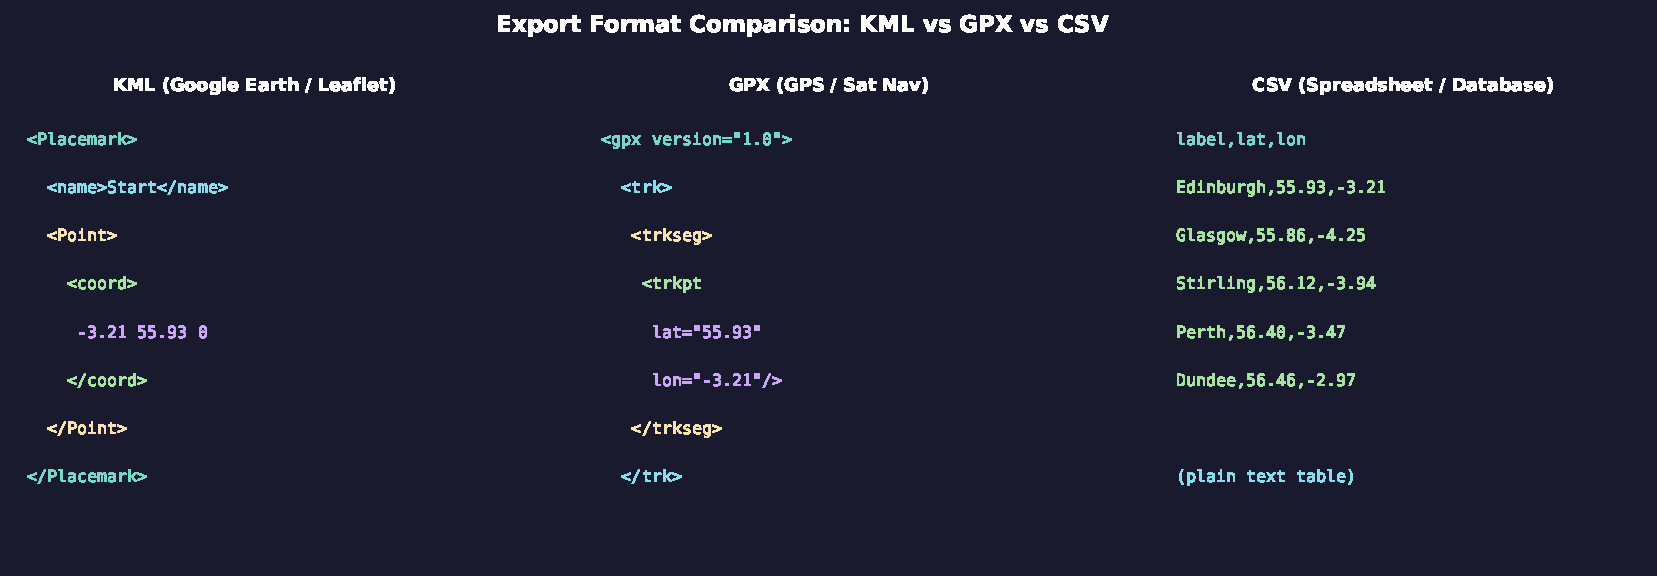
\includegraphics[width=0.92\textwidth]{fig_export_formats}
  \end{center}

  \medskip
  The three formats serve different audiences:
  \begin{itemize}
    \item \textbf{KML} for web mapping visualisation (planners, managers).
    \item \textbf{GPX} for drivers using GPS navigation devices.
    \item \textbf{CSV} for data analysts and business system integration.
  \end{itemize}

  \begin{alertblock}{Key Insight}
    Supporting multiple export formats does not require rewriting the export
    logic from scratch for each format.  The \emph{ExportService} interface
    pattern (next frame) means that the same route data can be written to
    all three formats with a single call to a factory method.
  \end{alertblock}

\end{frame}

%% ────────────────────────────────────────────────────────────
\begin{frame}[allowframebreaks]{9.4 The ExportService Interface}

  Just as the \texttt{Geocoder} interface allowed geocoder swapping,
  the \texttt{ExportService} interface unifies all export formats behind
  a single API.  The interface declares three operations:

  \begin{itemize}
    \item \texttt{addTrack(List<LatLon> locs)}: records a polyline (the route
          path) as a list of coordinates.
    \item \texttt{addWaypoint(LatLon loc, String caption, String desc)}:
          records a named point of interest (e.g., a delivery address).
    \item \texttt{write(String path, String name)}: writes the collected data
          to a file at the given path.
  \end{itemize}

  \begin{center}
    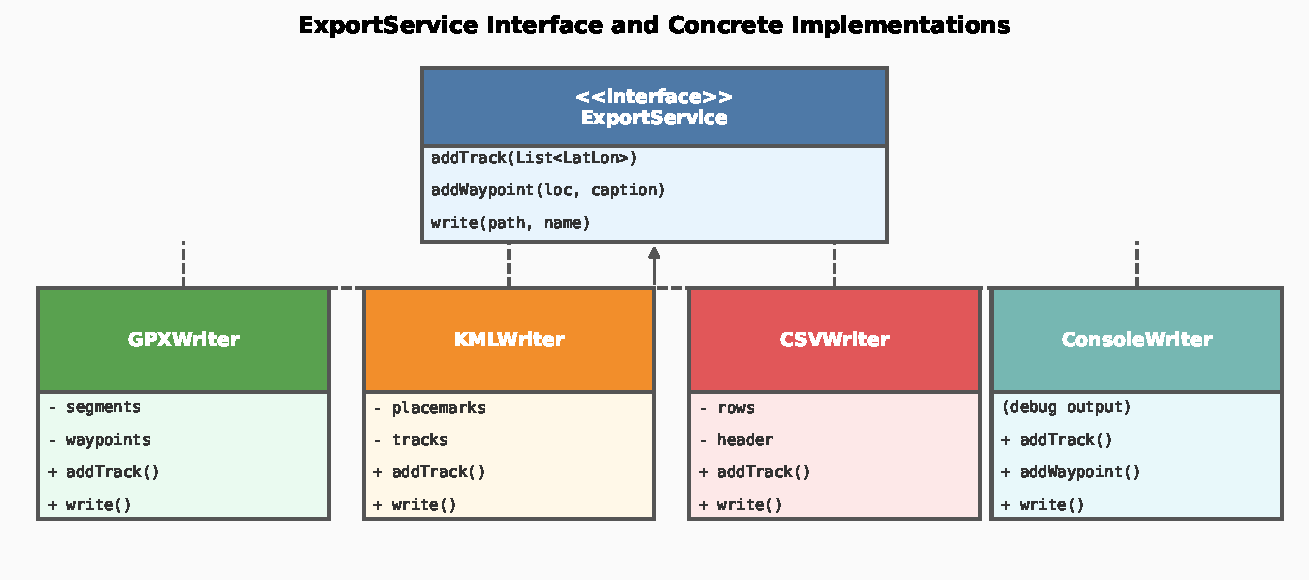
\includegraphics[width=0.88\textwidth]{fig_export_service}
  \end{center}

  \medskip
  Four concrete implementations are provided in the book:
  \texttt{GPXWriter}, \texttt{KMLWriter}, \texttt{CSVWriter}, and
  \texttt{ConsoleWriter} (for debugging).  All four implement
  \texttt{ExportService} so they can be used interchangeably.

  \framebreak

  \textbf{How the GPX Writer Works}

  \medskip
  A GPX file has the following overall structure:
  \begin{enumerate}
    \item An XML header identifying the GPX version and namespaces.
    \item Zero or more \texttt{<wpt>} (waypoint) elements, one per delivery stop.
    \item Zero or more \texttt{<trk>} (track) elements, each containing a
          \texttt{<trkseg>} (track segment) with a list of
          \texttt{<trkpt>} (track point) elements.
    \item An XML footer closing the root \texttt{<gpx>} element.
  \end{enumerate}

  The \texttt{GPXWriter} accumulates waypoints and track segments as
  strings in memory.  When \texttt{write()} is called, it concatenates
  the header, the waypoints, the track segments, and the footer into a
  single string and writes it to a file.

  \begin{exampleblock}{Complete Workflow: Route from Edinburgh to Fife}
    The following sequence (Listing~9.14 in the book) demonstrates
    the full pipeline in action:
    \begin{enumerate}
      \item Geocode \texttt{"10 Colinton Road, Edinburgh"} to get start
            coordinates.
      \item Geocode \texttt{"Scottish Vintage Bus Museum, Fife"} to get
            end coordinates.
      \item Call \texttt{GraphHopper.findRoute(start, end)} to get the road
            path.
      \item Call \texttt{export.addWaypoint(start, "Start", "Edinburgh Napier")}.
      \item Call \texttt{export.addWaypoint(end, "Destination", "Bus Museum")}.
      \item Call \texttt{export.addTrack(route.getPath())}.
      \item Call \texttt{export.write("out", "journey")}.
    \end{enumerate}
    The resulting file can be loaded into any GPX viewer to display the
    exact road-network route on an OSM base map.
  \end{exampleblock}

\end{frame}

%% ────────────────────────────────────────────────────────────
\begin{frame}[allowframebreaks]{9.4 Visualising the Result on a Map}

  Once the route is exported to KML or GPX, it can be overlaid on an
  OpenStreetMap base map using a web visualiser.

  The figure below shows an example GPX output (from the book's
  \texttt{ExportTest} demo) visualised using \texttt{gpxvisualizer.com}.
  The red line traces the road-network route from Edinburgh Napier University
  to the Scottish Vintage Bus Museum in Fife, including the Forth Road Bridge.

  \medskip
  \begin{center}
    % Cropped from book Fig. 9.2 (page 205)
    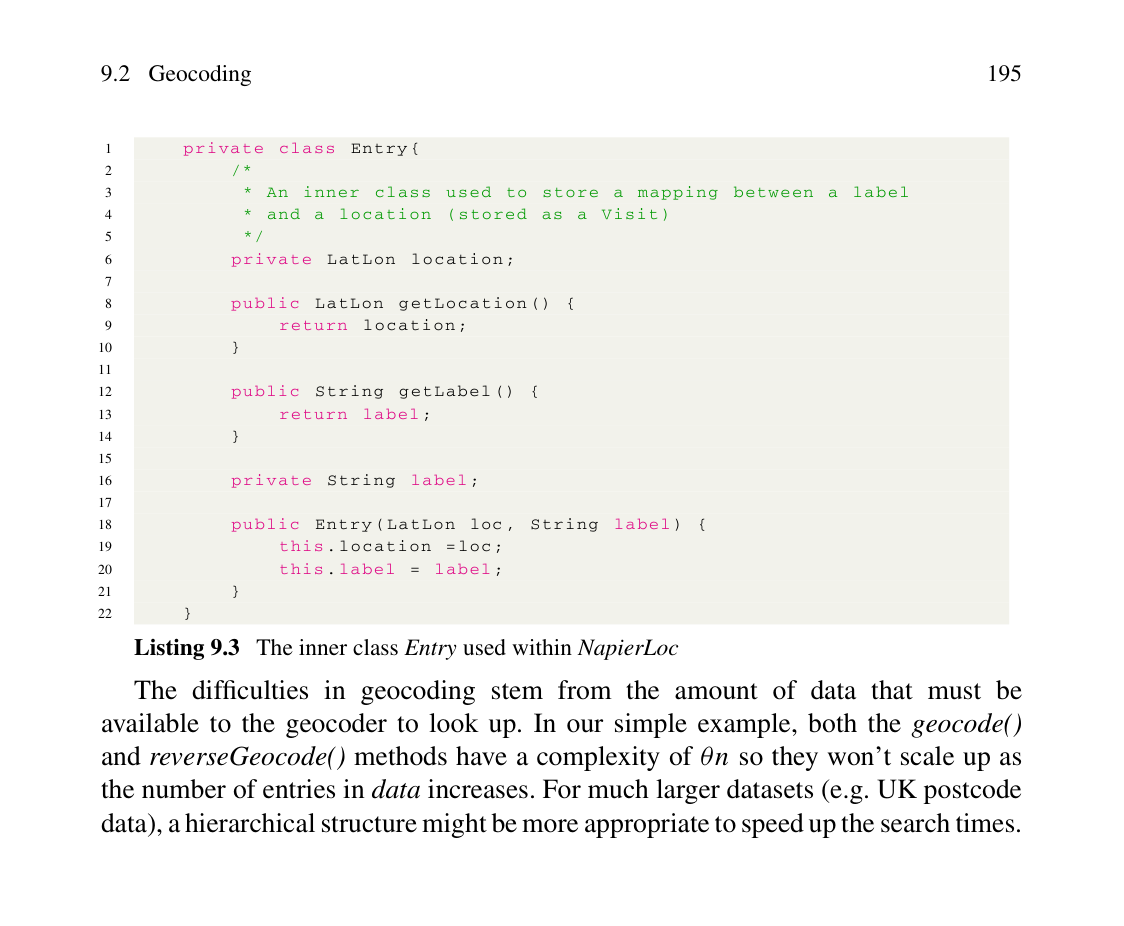
\includegraphics[width=0.75\textwidth]{fig_gpx_osm_map}
  \end{center}

  \medskip
  The blue markers indicate the start and end waypoints.  The underlying
  base map is provided by OSM.  This kind of visualisation is invaluable
  for sanity-checking an optimiser's output: it immediately reveals whether
  routes are geographically sensible.

  \framebreak

  \textbf{Schematic Route Visualisation}

  \medskip
  The following schematic illustrates the general concept of overlaying
  an optimised multi-stop delivery route on a map:

  \begin{center}
    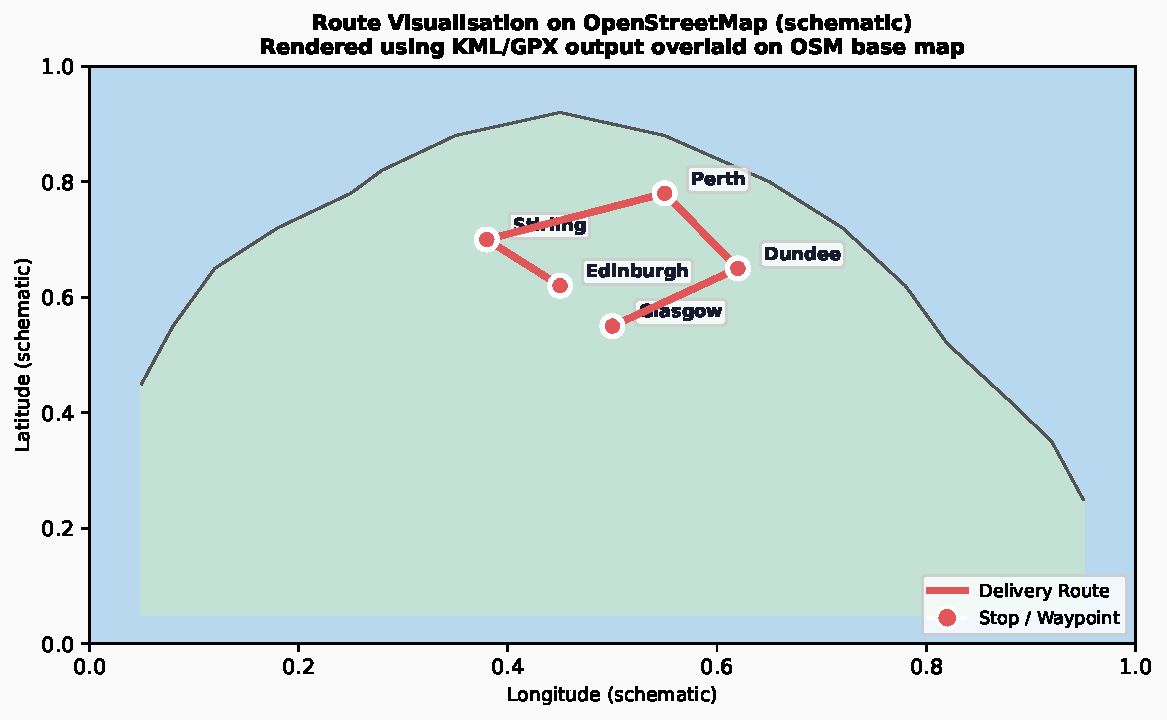
\includegraphics[width=0.72\textwidth]{fig_map_visualisation}
  \end{center}

  \begin{itemize}
    \item Each red circle represents a delivery stop (waypoint).
    \item The red connecting lines represent the road-network route between
          consecutive stops.
    \item The blue background represents water bodies (Firth of Forth, etc.).
    \item The green area represents land.
  \end{itemize}

  In a real deployment, this schematic would be replaced by actual OSM
  tile layers rendered in a browser using Leaflet (JavaScript) or Folium
  (Python wrapper around Leaflet).

\end{frame}

%% ────────────────────────────────────────────────────────────
\begin{frame}[fragile]{Python: Writing a KML File}

  The Python \texttt{simplekml} library makes it easy to create KML files
  for route visualisation.  The following example creates a KML file with
  two waypoints and a connecting line (representing a one-leg route).

\begin{lstlisting}[style=pycode, caption={Writing a KML file with simplekml}]
# pip install simplekml
import simplekml

def write_kml(waypoints: list, track: list, out_path: str, name: str):
    """
    Write a KML file with waypoints and a route track.

    waypoints : list of (lat, lon, label, description) tuples
    track     : list of (lat, lon) tuples defining the route path
    out_path  : directory to save the file
    name      : filename stem (no extension)
    """
    kml = simplekml.Kml()

    # Add waypoints (placemarks)
    for lat, lon, label, desc in waypoints:
        pnt = kml.newpoint(name=label, description=desc)
        pnt.coords = [(lon, lat)]   # KML uses (lon, lat) order!
        pnt.style.iconstyle.color = simplekml.Color.red
        pnt.style.iconstyle.scale = 1.2

    # Add track as a LineString
    if track:
        ls = kml.newlinestring(name=f"{name} route")
        ls.coords = [(lon, lat) for lat, lon in track]
        ls.style.linestyle.color  = simplekml.Color.blue
        ls.style.linestyle.width  = 4

    kml.save(f"{out_path}/{name}.kml")
    print(f"Saved KML: {out_path}/{name}.kml")

# --- Usage example ---
waypoints = [
    (55.9329, -3.2139, "Start",       "Edinburgh Napier University"),
    (56.1503, -3.3521, "Destination", "Scottish Vintage Bus Museum"),
]
# In a real application, 'track' would come from a routing service
track = [(55.9329, -3.2139), (55.9700, -3.2500),
         (56.0200, -3.3000), (56.1503, -3.3521)]

write_kml(waypoints, track, out_path="./output", name="delivery_route")
\end{lstlisting}

  \begin{alertblock}{Coordinate Order}
    KML (and GeoJSON) use \texttt{(longitude, latitude)} order, which is
    the \emph{opposite} of the mathematical convention \texttt{(latitude,
    longitude)}.  Always double-check coordinate order when writing
    geospatial files --- swapping lat and lon is one of the most common bugs.
  \end{alertblock}

\end{frame}

%% ────────────────────────────────────────────────────────────
\begin{frame}[fragile]{Python: Writing a GPX File}

  The \texttt{gpxpy} library provides a Pythonic interface for creating
  and reading GPX files.

\begin{lstlisting}[style=pycode, caption={Writing a GPX file with gpxpy}]
# pip install gpxpy
import gpxpy
import gpxpy.gpx

def write_gpx(waypoints: list, track: list, out_path: str, name: str):
    """
    Write a GPX file with named waypoints and a route track.

    waypoints : list of (lat, lon, name, description) tuples
    track     : list of (lat, lon) tuples
    """
    gpx = gpxpy.gpx.GPX()

    # Add waypoints
    for lat, lon, wpt_name, desc in waypoints:
        wpt = gpxpy.gpx.GPXWaypoint(
            latitude=lat, longitude=lon,
            name=wpt_name, description=desc
        )
        gpx.waypoints.append(wpt)

    # Add track segment
    gpx_track = gpxpy.gpx.GPXTrack(name=name)
    gpx.tracks.append(gpx_track)
    segment = gpxpy.gpx.GPXTrackSegment()
    gpx_track.segments.append(segment)

    for lat, lon in track:
        segment.points.append(
            gpxpy.gpx.GPXTrackPoint(latitude=lat, longitude=lon)
        )

    with open(f"{out_path}/{name}.gpx", "w") as f:
        f.write(gpx.to_xml())
    print(f"Saved GPX: {out_path}/{name}.gpx")

# --- Usage ---
waypoints = [
    (55.9329, -3.2139, "Start",       "Edinburgh Napier University"),
    (56.1503, -3.3521, "Destination", "Scottish Vintage Bus Museum"),
]
track = [(55.9329, -3.2139), (56.0200, -3.2800), (56.1503, -3.3521)]
write_gpx(waypoints, track, out_path="./output", name="delivery_route")
\end{lstlisting}

\end{frame}

%% ────────────────────────────────────────────────────────────
\begin{frame}[fragile]{Python: Writing a CSV File and Visualising with Folium}

  CSV export is the simplest format and is achieved with Python's built-in
  \texttt{csv} module.  Folium wraps the Leaflet.js mapping library,
  allowing routes to be displayed on an interactive OSM base map saved as
  an HTML file.

\begin{lstlisting}[style=pycode, caption={CSV export and interactive map with Folium}]
import csv, os
# pip install folium
import folium

def write_csv(waypoints, out_path, name):
    """Write waypoints to a CSV file."""
    with open(f"{out_path}/{name}.csv", "w", newline="") as f:
        writer = csv.writer(f)
        writer.writerow(["label", "latitude", "longitude"])
        for lat, lon, label, *_ in waypoints:
            writer.writerow([label, lat, lon])
    print(f"Saved CSV: {out_path}/{name}.csv")

def write_folium_map(waypoints, track, out_path, name):
    """Create an interactive Leaflet map using Folium."""
    # Centre the map on the mean of all waypoints
    centre_lat = sum(w[0] for w in waypoints) / len(waypoints)
    centre_lon = sum(w[1] for w in waypoints) / len(waypoints)

    m = folium.Map(location=[centre_lat, centre_lon], zoom_start=10,
                   tiles="OpenStreetMap")

    # Add waypoint markers
    for lat, lon, label, *_ in waypoints:
        folium.Marker(
            location=[lat, lon],
            popup=label,
            icon=folium.Icon(color="red", icon="info-sign"),
        ).add_to(m)

    # Add the route as a polyline
    if track:
        folium.PolyLine(track, color="blue", weight=4,
                        opacity=0.8).add_to(m)

    m.save(f"{out_path}/{name}.html")
    print(f"Saved interactive map: {out_path}/{name}.html")

# --- Usage ---
waypoints = [
    (55.9329, -3.2139, "Edinburgh Napier"),
    (56.1503, -3.3521, "Bus Museum, Fife"),
]
track = [(55.9329, -3.2139), (56.0200, -3.2800), (56.1503, -3.3521)]
os.makedirs("./output", exist_ok=True)
write_csv(waypoints, "./output", "route")
write_folium_map(waypoints, track, "./output", "route")
\end{lstlisting}

\end{frame}

%% ============================================================
\section{9.5 Conclusions}
%% ============================================================

\begin{frame}[allowframebreaks]{9.5 Conclusions}

  This chapter has shown how a nature-inspired optimisation algorithm can
  be connected to real-world geographic data sources and services.  The
  key accomplishment is bridging the gap between the abstract mathematical
  world of optimisation (where locations are just indices 0 to $n-1$ in a
  distance matrix) and the physical world (where locations have addresses,
  coordinates, and road connections).

  \begin{block}{Summary of Tools and Their Roles}
    \centering
    \renewcommand{\arraystretch}{1.3}
    \begin{tabular}{>{\bfseries}p{2.6cm} p{4.4cm} p{4.0cm}}
      \toprule
      \textbf{Tool} & \textbf{Purpose} & \textbf{Open Alternatives} \\
      \midrule
      Nominatim & Forward/reverse geocoding & Google Maps API \\
      GraphHopper & Local routing (offline) & OSRM, Valhalla \\
      OSRM / ORS & Web routing API & Google Directions API \\
      KML writer & Map visualisation export & GeoJSON \\
      GPX writer & GPS / Sat Nav export & TCX, FIT \\
      CSV writer & Spreadsheet/DB export & JSON, Parquet \\
      Folium & Interactive HTML maps & Leaflet.js, MapLibre \\
      \bottomrule
    \end{tabular}
  \end{block}

  \framebreak

  \textbf{The Significance of OpenStreetMap}

  \medskip
  Possibly the most important development enabling this chapter is the growth
  of OpenStreetMap (OSM) as a freely available, community-maintained
  geographic database.  Before OSM, access to high-quality road-network
  data required expensive commercial licences that put real-world routing
  out of reach for academic researchers and small companies.  OSM changed
  this fundamentally.

  Building on OSM, the following open-source ecosystem has emerged:
  \begin{itemize}
    \item \textbf{Nominatim}: free geocoding for any address in OSM.
    \item \textbf{GraphHopper} and \textbf{OSRM}: fast local routing engines
          built on OSM road data.
    \item \textbf{Leaflet}, \textbf{OpenLayers}: web mapping libraries that
          display OSM tiles in browsers.
    \item \textbf{Folium}: a Python library wrapping Leaflet for rapid
          prototyping.
    \item \textbf{QGIS}: a full open-source GIS desktop application for
          spatial analysis.
  \end{itemize}

  \begin{alertblock}{Key Takeaway}
    The design patterns used in this chapter --- interfaces for geocoders
    and routing engines, caching decorators, and a unified export service ---
    make it straightforward to swap one provider for another as requirements
    change.  A solver built with these patterns can be tested with a small,
    hard-coded geocoder and then deployed against Nominatim or Google Maps
    with minimal code changes.
  \end{alertblock}

  \framebreak

  \textbf{References}

  \begin{itemize}
    \item Haklay, M., and P.\ Weber.\ 2008.\ OpenStreetMap: user-generated
          street maps.\ \textit{IEEE Pervasive Computing} 7(4): 12--18.
    \item Nominatim.\ 2021.\ \url{https://nominatim.org/}
    \item GraphHopper GmbH.\ 2021.\ GraphHopper Directions API.\
          \url{https://github.com/graphhopper/graphhopper}
    \item OGC.\ 2015.\ KML 2.3.\
          \url{http://docs.opengeospatial.org/is/12-007r2/12-007r2.html}
    \item Overview --- Nominatim Documentation.\ 2020.\
          \url{https://nominatim.org/release-docs/develop/api/Overview/}
    \item Vladimir Agafonkin.\ 2020.\ Leaflet (open-source mapping library).
    \item Foundation, O.K.\ 2021.\ Global Open Data Index: Locations.\
          \url{https://index.okfn.org/dataset/postcodes/}
    \item Google Maps.\ 2021.\ \url{https://www.google.com/maps/}
  \end{itemize}

\end{frame}

%% ============================================================
%% Appendix: Complete Python Examples
%% ============================================================
\appendix
\section*{Appendix: Complete Python Examples}

\begin{frame}[fragile]{Python: Full End-to-End Pipeline}

  The following script ties together geocoding, routing, and export into a
  single demonstration.  It geocodes two addresses, queries OSRM for the
  route, and writes KML and CSV output files.

\begin{lstlisting}[style=pycode, caption={End-to-end: geocode + route + export}]
from geopy.geocoders import Nominatim
from geopy.extra.rate_limiter import RateLimiter
import requests, os

geolocator = Nominatim(user_agent="ch9_demo_pipeline")
geocode = RateLimiter(geolocator.geocode, min_delay_seconds=1)

# 1. Geocode two addresses
start_addr = "10 Colinton Road, Edinburgh"
end_addr   = "Scottish Vintage Bus Museum, Fife"

start_loc = geocode(start_addr)
end_loc   = geocode(end_addr)
s = (start_loc.latitude, start_loc.longitude)
e = (end_loc.latitude,   end_loc.longitude)
print(f"Start: {s}   End: {e}")

# 2. Get route from OSRM (single route, with geometry)
coord_str = f"{s[1]},{s[0]};{e[1]},{e[0]}"
url = (f"http://router.project-osrm.org/route/v1/driving/{coord_str}"
       f"?overview=full&geometries=geojson")
data = requests.get(url, timeout=15).json()
path_coords = data["routes"][0]["geometry"]["coordinates"]
# OSRM returns [lon, lat]; convert to [lat, lon]
track = [(c[1], c[0]) for c in path_coords]
dist_km  = data["routes"][0]["distance"] / 1000.0
time_min = data["routes"][0]["duration"] / 60.0
print(f"Route: {dist_km:.1f} km, {time_min:.1f} min")

# 3. Export to CSV
os.makedirs("output", exist_ok=True)
import csv
with open("output/route.csv", "w", newline="") as f:
    w = csv.writer(f)
    w.writerow(["label", "lat", "lon"])
    w.writerow(["Start", s[0], s[1]])
    w.writerow(["End",   e[0], e[1]])
print("Pipeline complete. Files in ./output/")
\end{lstlisting}

\end{frame}

%% ────────────────────────────────────────────────────────────
\begin{frame}[fragile]{Python: OpenRouteService (ORS) --- Directions API}

  OpenRouteService (ORS) is a free alternative to OSRM with an easy-to-use
  Python client.  An API key is required (free tier available).

\begin{lstlisting}[style=pycode, caption={Routing with OpenRouteService Python client}]
# pip install openrouteservice
import openrouteservice as ors

# Replace with your ORS API key from https://openrouteservice.org/
client = ors.Client(key="YOUR_API_KEY_HERE")

coords = [
    [-3.2139, 55.9329],   # Edinburgh Napier  (lon, lat)
    [-3.9369, 56.1165],   # Stirling          (lon, lat)
    [-3.4370, 56.3964],   # Perth             (lon, lat)
    [-2.9707, 56.4621],   # Dundee            (lon, lat)
]

# Request a route visiting all coords in order (car driving)
route = client.directions(
    coordinates=coords,
    profile="driving-car",
    format="geojson",
)

# Extract summary
summary = route["features"][0]["properties"]["summary"]
print(f"Total distance: {summary['distance']/1000:.1f} km")
print(f"Total duration: {summary['duration']/60:.1f} min")

# Extract waypoints for export
geometry = route["features"][0]["geometry"]["coordinates"]
track = [(c[1], c[0]) for c in geometry]   # (lon,lat) -> (lat,lon)
print(f"Route has {len(track)} waypoints")

# --- Distance Matrix with ORS ---
matrix = client.distance_matrix(
    locations=coords,
    profile="driving-car",
    metrics=["distance", "duration"],
    units="km",
)
print("\nDistance matrix (km):")
for row in matrix["distances"]:
    print([f"{v:6.1f}" for v in row])
\end{lstlisting}

\end{frame}

%% ────────────────────────────────────────────────────────────
\begin{frame}[allowframebreaks]{Summary: Chapter 9 Key Points}

  This chapter covered the three pillars of connecting optimisation to the
  real world.  Here is a concise summary of what was learned:

  \textbf{Geocoding (Section~9.2)}
  \begin{itemize}
    \item Geocoding converts addresses to $(lat, lon)$ coordinates; reverse
          geocoding does the opposite.
    \item Nominatim (free, OSM-based) is a practical choice for research and
          small-scale deployment.
    \item Caching is essential to avoid redundant web requests and to respect
          rate limits.
    \item The \texttt{Geocoder} interface allows any geocoder to be swapped
          without changing the optimiser code.
  \end{itemize}

  \textbf{Routing Services (Section~9.3)}
  \begin{itemize}
    \item Routing services compute actual road-network distances and travel
          times, which are significantly more accurate than straight-line
          approximations.
    \item The distance matrix ($D_{ij}$: distance from location $i$ to $j$)
          should be pre-computed and cached before the optimiser runs.
    \item GraphHopper enables offline routing; OSRM and ORS provide web APIs.
    \item The \texttt{RoutingEngine} abstract class makes routing back-ends
          swappable.
  \end{itemize}

  \textbf{Exporting Data (Section~9.4)}
  \begin{itemize}
    \item KML and GPX are XML-based geospatial formats for visualisation
          and navigation respectively.
    \item CSV is the simplest format for business system integration.
    \item The \texttt{ExportService} interface pattern allows writing to
          multiple formats with one common API.
    \item Folium (Python) creates interactive web maps from route data with
          minimal code.
  \end{itemize}

  \framebreak

  \begin{center}
    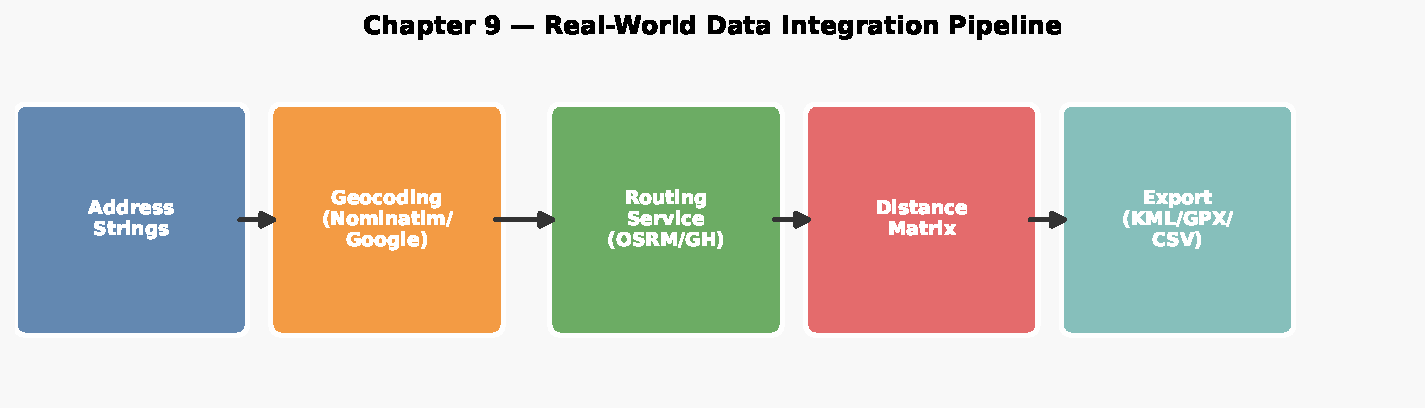
\includegraphics[width=0.88\textwidth]{fig_pipeline}
  \end{center}

  \begin{alertblock}{Final Takeaway}
    The emergence of OpenStreetMap and the open-source tools built on top of
    it has removed the geographic data barrier that once made real-world
    delivery optimisation inaccessible to researchers and small organisations.
    Combining a nature-inspired optimiser with Nominatim (geocoding),
    GraphHopper (routing), and Folium (visualisation) gives a complete,
    free, and practical solver for real delivery problems --- with results
    that can be exported directly to a driver's GPS device.
  \end{alertblock}

\end{frame}

\end{document}
